\documentclass[compress]{beamer}
\usepackage{ifthen,verbatim}

\setbeamertemplate{navigation symbols}{}

\begin{document}

\begin{frame}
\frametitle{Muon HIP Alignment CSA07 Plan}
\begin{itemize}
\item We want to study the effect of QCD muons on alignment by
repeating the alignment process on realistic soups with different $p_T$ cuts
\item Three cuts: 20~GeV, 30~GeV, 40~GeV $\to$ 30~GB total
\item Align each of the three samples times two modes (globalMuon,
standAloneMuon) times three subdivisions of the data for dependence on
statistics (90\%, 9\%, and 1\%)
\item Order of operations in each study:

\begin{enumerate}
\item Wheel/disk alignment with a 1000 events: well under an hour
\item 1 globalMuon iteration (12 hours) concurrent with 7 standalone
iterations (12 hours when divided into 7 subsamples): 8$\times$9 = 72 jobs
\item CSC layer alignment, same conditions: 12 hours, 72 jobs
\end{enumerate}

\item (Second globalMuon iteration for checking residuals is in the CSC
layer alignment)

\item Maximum of 72 jobs for a total of 25 hours with 81$\times$14~MB + 81$\times$80~MB = 7~GB of histogram output
\end{itemize}
\end{frame}

\begin{frame}
\frametitle{Determination of the $p_T$ cut (biggest $\mu$ $p_T$ in the event)}

\vspace{-0.35 cm}
\begin{columns}
\column{0.5\linewidth}
\begin{center}
QCDmu muons in semilog scale

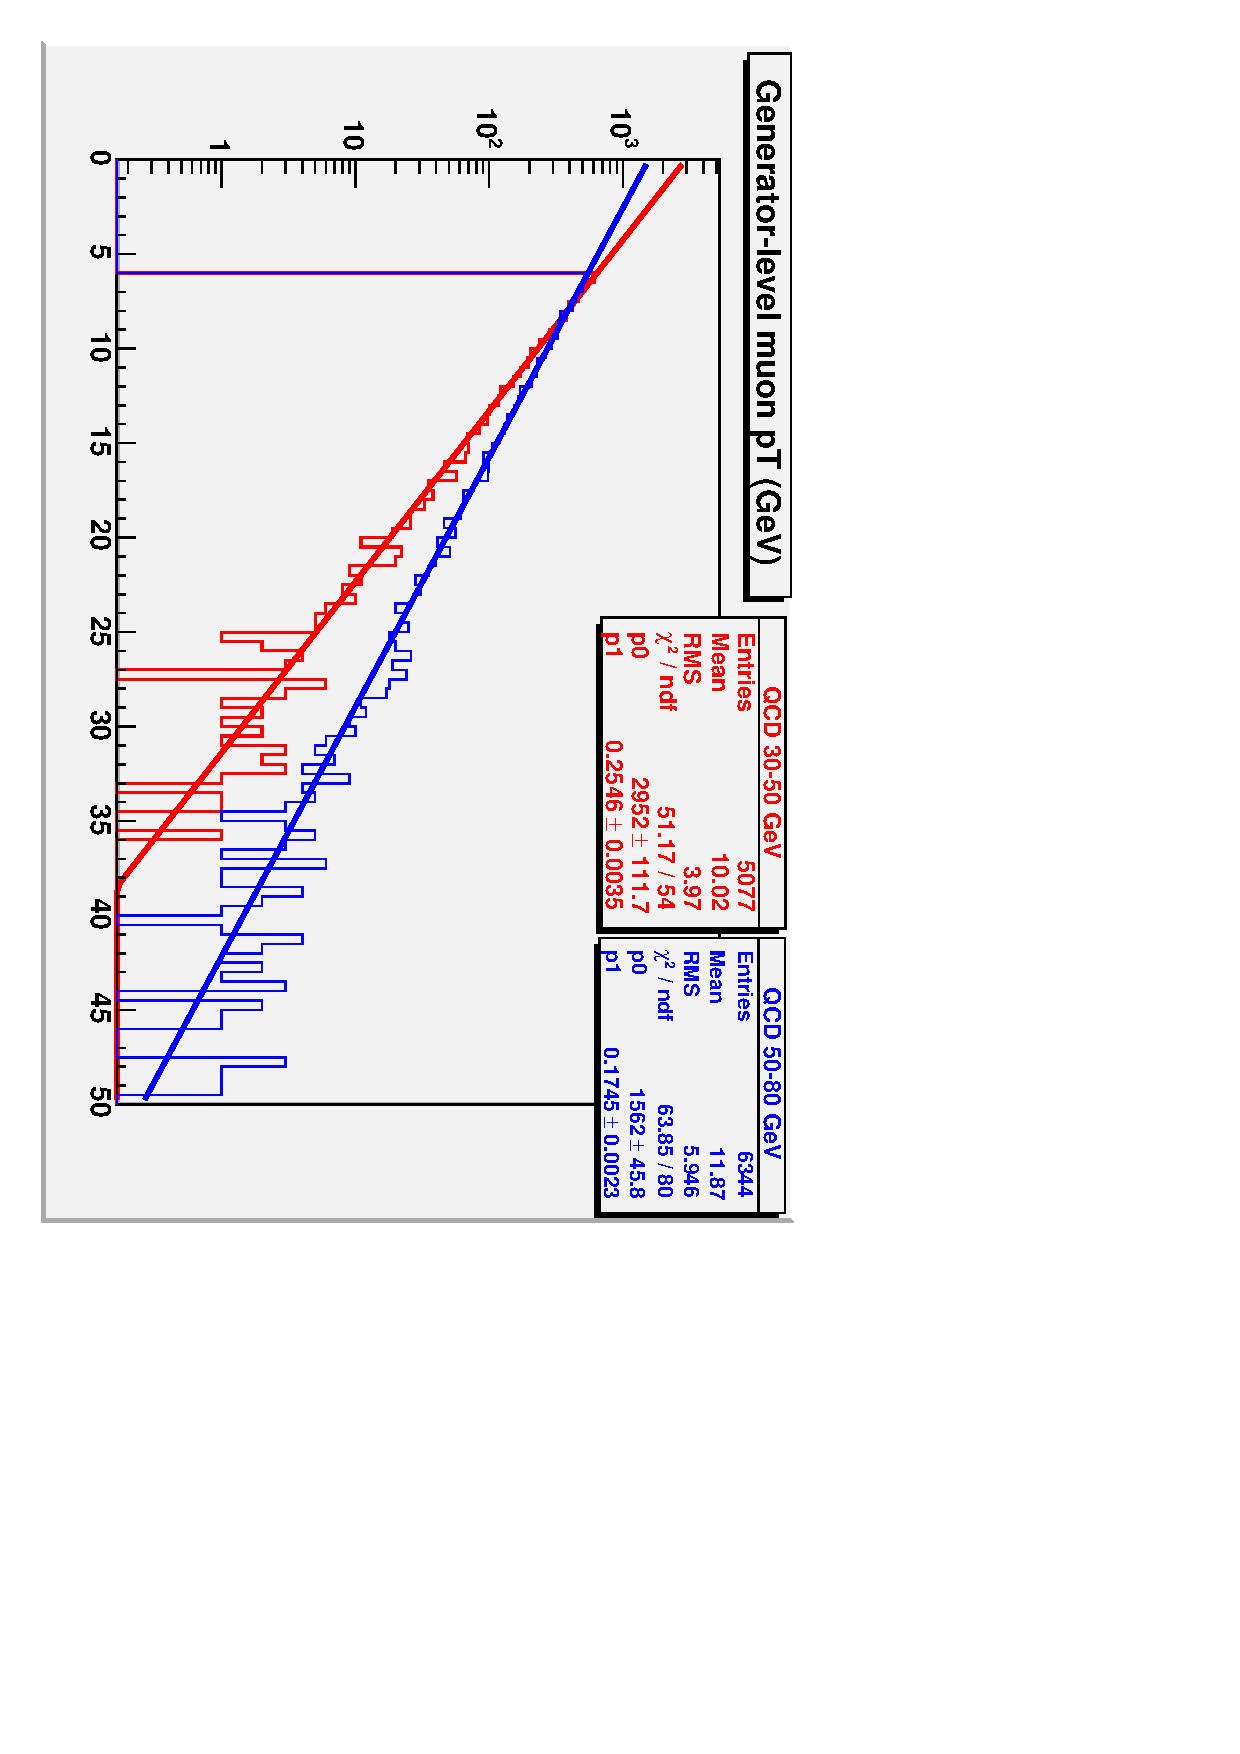
\includegraphics[height=\linewidth, angle=90]{exponential_qcd.pdf}
\end{center}

\column{0.5\linewidth}
\begin{center}
$W$ + $Z$ in linear scale

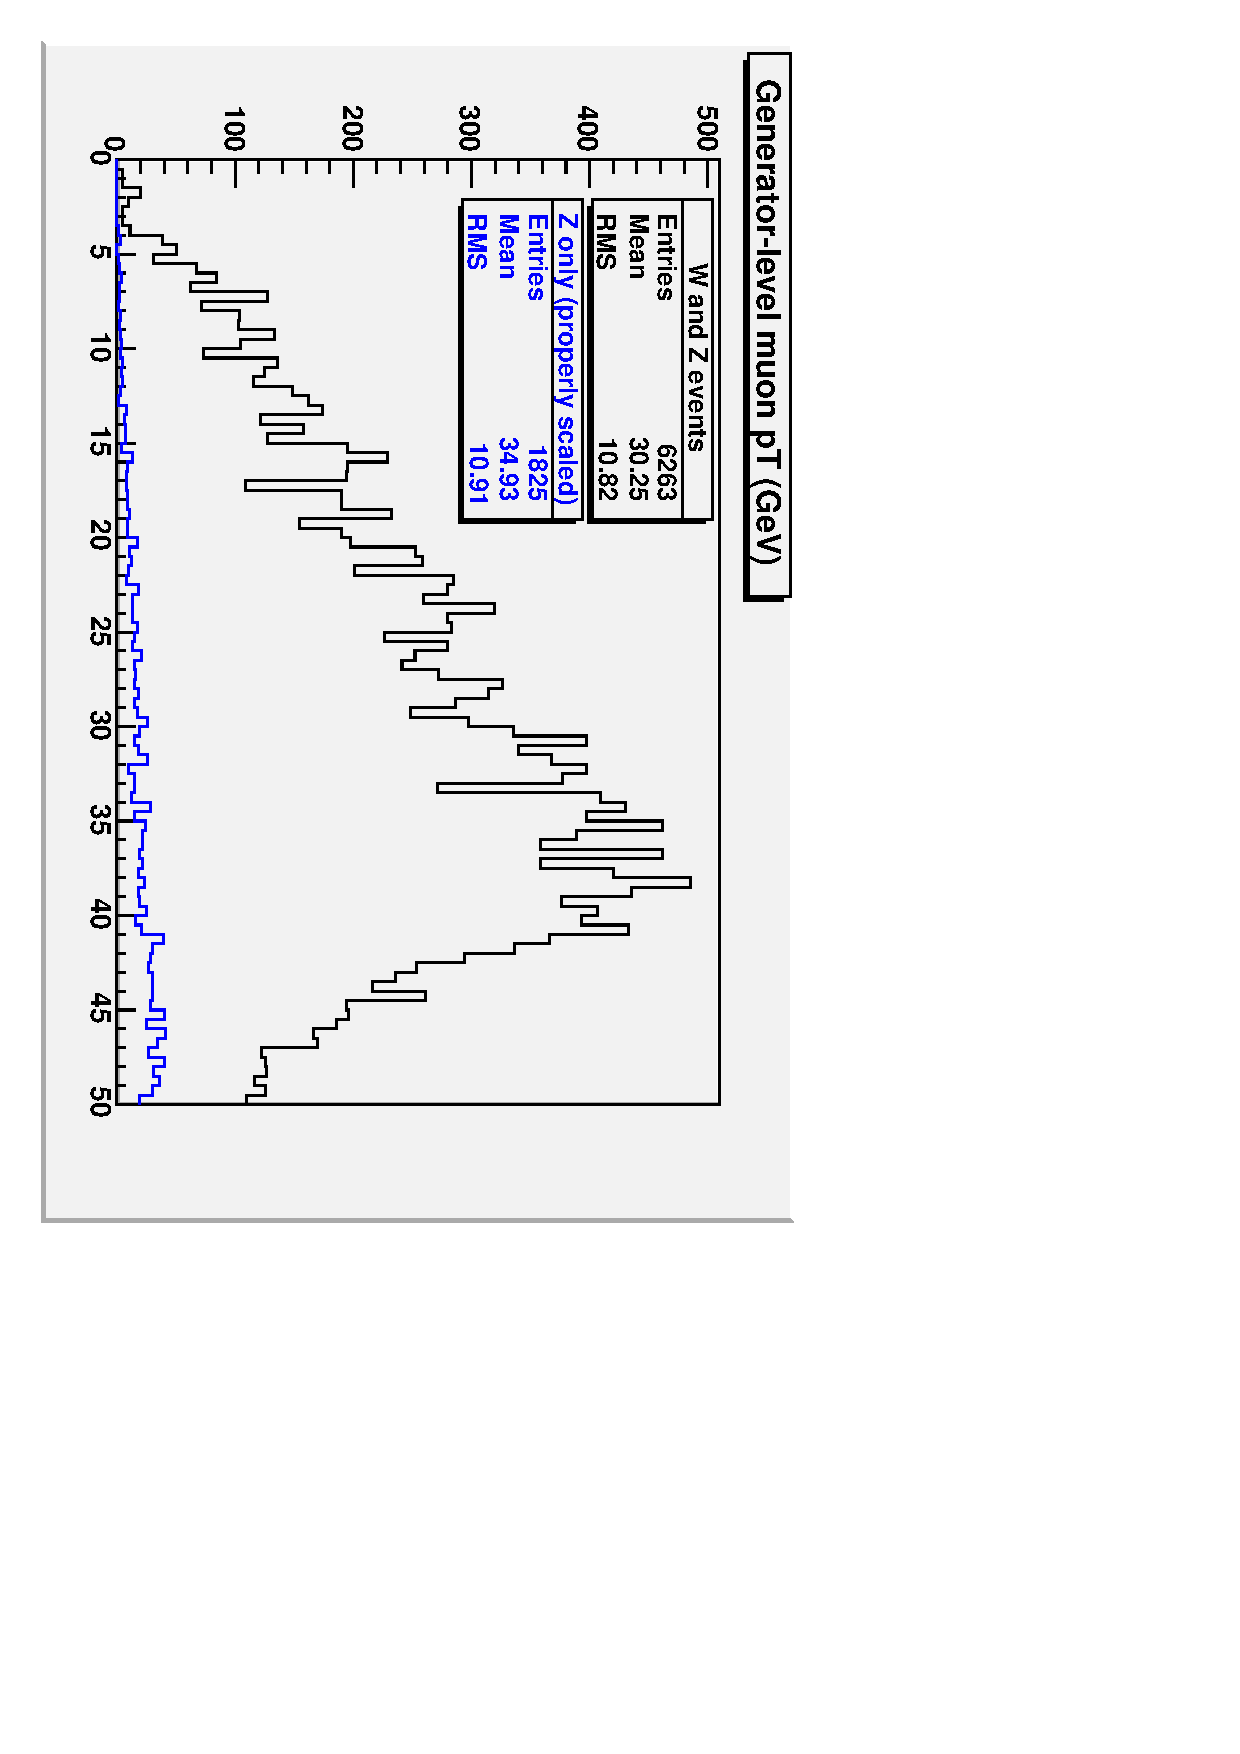
\includegraphics[height=\linewidth, angle=90]{w_and_z.pdf}
\end{center}
\end{columns}

\begin{center}
\small
We always want $\sim$100k $W$ + $Z$ events, so that sets the normalization

AlCaRecoMu = 17 kB/muon due to two copies of RecHits

\begin{tabular}{c c c c c}
\hline\hline & $p_T$ cut & events & disk space & alignment time/iteration \\\hline
& 10 GeV & 6.1 million & 130 GB & 76.3 hours \\
& 15 GeV & 2.3 million & 48 GB & 28.7 hours \\
$\to$ & 20 GeV & 0.94 million & 21 GB & 11.8 hours \\
& 25 GeV & 0.45 million & 9.4 GB & 5.6 hours \\
$\to$ & 30 GeV & 0.25 million & 5.2 GB & 3.1 hours \\
& 35 GeV & 0.17 million & 3.6 GB & 2.1 hours \\
$\to$ & 40 GeV & 0.14 million & 3.0 GB & 1.8 hours \\\hline\hline
\end{tabular}
\end{center}
\end{frame}

\begin{frame}
\frametitle{Conditions for the samples}
\begin{itemize}\setlength{\itemsep}{0.25 cm}
\item Source of QCD muons: {\tt QCDmu\_Pt\_30\_50} through {\tt QCDmu\_Pt\_170\_230} in the correct proportions
\item Three statistically independent samples: {\it different} events
\item Miscalibrated chambers (10~pb$^{-1}$ scenario)
\item Realistically misaligned tracker (10~pb$^{-1}$ scenario)
\item Wheels/disks misaligned 3~mm and 1~mrad in all directions/angles
\item Chambers misaligned 3~mm and 1~mrad in all directions/angles
\item CSC layers misaligned 191~$\mu$m in $x$, 335~$\mu$m in $y$ and 0.04~mrad in $\phi_z$
\item No DT layer/superlayer misalignment
\end{itemize}
\end{frame}

\begin{frame}
\frametitle{Basic questions}
\begin{itemize}\setlength{\itemsep}{0.5 cm}
\item Do I write all of the scripts and submit them myself?  Who presses the ``go'' button?
\item We can use AlignmentMuonSelectorModule to apply the $p_T$ cuts,
but with a second invocation and outside the .cff file.  Is this
allowed?
\begin{center}
MuonSelectorLabel1 (in .cff, no $p_T$ cut)

$\downarrow$

MuonSelectorLabel2 (in .cfg, apply $p_T$ cut)

$\downarrow$

disk
\end{center}

\end{itemize}
\end{frame}

\end{document}
